% Annexes

\section*{Annexes}

\addcontentsline{toc}{section}{Annexes}



\subsection*{Annexe A : Schéma de la Base de Données Drizzle ORM}

\addcontentsline{toc}{subsection}{Annexe A : Schéma de la Base de Données}



Cette annexe présente un extrait du schéma Drizzle ORM (\texttt{src/lib/db/schema.ts}) illustrant la structure des tables principales.



\begin{codebox}

\begin{lstlisting}

// Tables Better Auth (authentification)

export const user = pgTable("user", {

  id: text("id").primaryKey(),

  name: text("name"),

  email: text("email").notNull().unique(),

  emailVerified: boolean("email_verified").default(false),

  image: text("image"),

  createdAt: timestamp("created_at").defaultNow(),

  updatedAt: timestamp("updated_at").defaultNow(),

});



export const session = pgTable("session", {

  id: text("id").primaryKey(),

  userId: text("user_id").notNull().references(() => user.id),

  token: text("token").notNull().unique(),

  expiresAt: timestamp("expires_at").notNull(),

});



export const account = pgTable("account", {

  id: text("id").primaryKey(),

  userId: text("user_id").notNull().references(() => user.id),

  accountId: text("account_id").notNull(),

  providerId: text("provider_id").notNull(),

});



export const verification = pgTable("verification", {

  id: text("id").primaryKey(),

  identifier: text("identifier").notNull(),

  value: text("value").notNull(),

  expiresAt: timestamp("expires_at").notNull(),

});



// Table profile (1:1 avec user)

export const profile = pgTable("profile", {

  id: serial("id").primaryKey(),

  userId: text("user_id").notNull().references(() => user.id).unique(),

  displayName: text("display_name"),

  bio: text("bio"),

  website: text("website"),

  twitter: text("twitter"),

  github: text("github"),

  avatarUrl: text("avatar_url"),

});



// Table launch (produit SaaS)

export const launch = pgTable("launch", {

  id: serial("id").primaryKey(),

  makerId: text("maker_id").notNull().references(() => user.id),

  title: text("title").notNull(),

  description: text("description"),

  logoUrl: text("logo_url"),

  upvoteCount: integer("upvote_count").default(0),

  createdAt: timestamp("created_at").defaultNow(),

});



// Table category

export const category = pgTable("category", {

  id: serial("id").primaryKey(),

  name: text("name").notNull(),

  slug: text("slug").notNull().unique(),

});



// Table plan (Free / Pro)

export const plan = pgTable("plan", {

  id: serial("id").primaryKey(),

  name: text("name").notNull(),

  priceMonthly: integer("price_monthly"),

  priceYearly: integer("price_yearly"),

  stripeProductId: text("stripe_product_id"),

  stripeMonthlyPriceId: text("stripe_monthly_price_id"),

  stripeYearlyPriceId: text("stripe_yearly_price_id"),

});



// Table subscription

export const subscription = pgTable("subscription", {

  id: serial("id").primaryKey(),

  userId: text("user_id").notNull().references(() => user.id).unique(),

  planId: integer("plan_id").notNull().references(() => plan.id),

  status: text("status").notNull().default("active"),

  stripeCustomerId: text("stripe_customer_id"),

  stripeSubscriptionId: text("stripe_subscription_id"),

});

\end{lstlisting}

\end{codebox}



\newpage



\subsection*{Annexe B : Structure du Projet}

\addcontentsline{toc}{subsection}{Annexe B : Structure du Projet}



\begin{codebox}

\begin{lstlisting}

marketplace-saas/ (12 166 LOC, 108 fichiers)

|-- e2e/                        (33 LOC)

|   |-- homepage.spec.ts

|-- public/

|   |-- uploads/launches/

|-- src/

|   |-- app/                    (3 198 LOC)

|   |   |-- layout.tsx

|   |   |-- page.tsx

|   |   |-- about/, api/, contact/, feed/

|   |   |-- forgot-password/, launch/, login/

|   |   |-- marketplace/, messages/, my-launches/

|   |   |-- new/, notifications/, pricing/

|   |   |-- privacy/, profile/, reset-password/

|   |   |-- settings/, signup/, terms/

|   |-- components/             (5 234 LOC)

|   |   |-- auth/, dev/, feed/, launch/

|   |   |-- marketplace/, providers/, ui/

|   |-- hooks/

|   |-- lib/                    (2 957 LOC)

|   |   |-- actions/            (Server Actions)

|   |   |-- db/

|   |   |   |-- migrations/     (4 migrations)

|   |   |   |   |-- 0000_remarkable_carnage.sql

|   |   |   |   |-- 0001_cuddly_namora.sql

|   |   |   |   |-- 0002_add_logo_url_to_launch.sql

|   |   |   |   |-- 0003_groovy_hannibal_king.sql

|   |   |   |-- schema.ts       (20 tables)

|   |   |   |-- index.ts

|   |   |-- auth.ts, auth-client.ts

|   |   |-- cache.ts, subscription.ts

|   |   |-- upload.ts, utils.ts

|   |   |-- *.test.ts           (11 fichiers de test)

|   |-- test/                   (111 LOC)

|   |-- types/

|-- next.config.ts

|-- package.json

|-- tsconfig.json

|-- vitest.config.ts

|-- playwright.config.ts

|-- drizzle.config.ts

|-- docker-compose.test.yml

\end{lstlisting}

\end{codebox}



\newpage



\subsection*{Annexe C : Dépendances Principales}

\addcontentsline{toc}{subsection}{Annexe C : Dépendances Principales}



\begin{table}[H]

\centering

\caption{Dépendances principales du projet SaaS Directory}

\label{tab:deps}

\begin{tabular}{@{}lll@{}}

\toprule

\textbf{Dépendance} & \textbf{Version} & \textbf{Description} \\

\midrule

next & 16.2.4 & Framework React avec App Router \\

react & 19.2.4 & Bibliothèque UI \\

react-dom & 19.2.4 & Rendu DOM React \\

drizzle-orm & 0.45.2 & ORM type-safe pour PostgreSQL \\

better-auth & 1.6.9 & Authentification OAuth + 2FA \\

pg & 8.20.0 & Driver PostgreSQL \\

@tanstack/react-query & 5.100.9 & Gestion de cache et requêtes \\

zod & 4.4.3 & Validation de schémas \\

framer-motion & 12.38.0 & Animations React \\

ioredis & 5.10.1 & Client Redis \\

resend & 6.12.2 & Service d'envoi d'emails \\

sonner & 2.0.7 & Notifications toast UI \\

tailwindcss & 4.0.0 & Framework CSS utilitaire \\

typescript & 5.7.0 & Typage statique \\

vitest & 4.1.5 & Tests unitaires et d'intégration \\

@playwright/test & 1.59.1 & Tests end-to-end \\

eslint & 9.0.0 & Linting du code \\

eslint-config-next & 16.2.4 & Règles ESLint Next.js \\

\bottomrule

\end{tabular}

\end{table}



\newpage



\subsection*{Annexe D : Diagramme de Déploiement}

\addcontentsline{toc}{subsection}{Annexe D : Diagramme de Déploiement}



\begin{figure}[H]

\centering

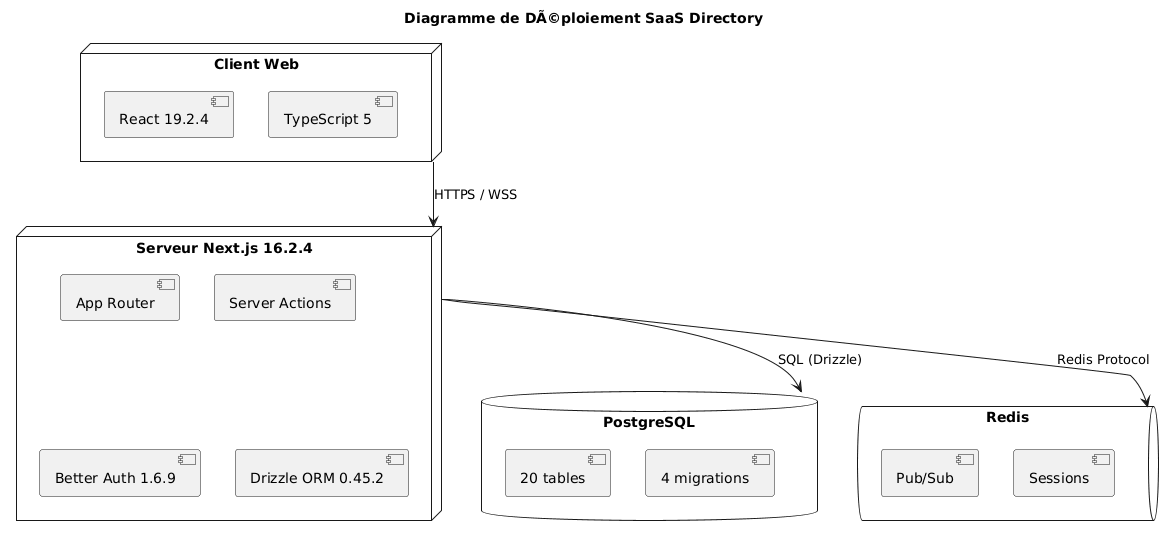
\includegraphics[width=0.95\textwidth]{assets/deployment.png}

\caption{Diagramme de Déploiement — Architecture Physique de SaaS Directory}

\label{fig:deployment}

\end{figure}



La figure~\ref{fig:deployment} décrit l'architecture physique du système et la répartition des artefacts logiciels sur les nÅ“uds matériels. SaaS Directory repose sur une architecture cloud-native distribuée sur trois environnements principaux : le client web (navigateur), la plateforme serverless (Next.js 16.2.4), et les services de données (PostgreSQL + Redis).



Le client web (React 19.2.4 / TypeScript 5) s'exécute dans le navigateur et communique avec les fonctions serverless via HTTPS. Les Server Actions Next.js 16.2.4 interagissent avec la base de données PostgreSQL via Drizzle ORM 0.45.2. Le système de messagerie temps réel utilise Redis Pub/Sub pour la diffusion des messages entre les instances serverless. L'authentification est assurée par Better Auth 1.6.9. Cette architecture sans serveur offre une scalabilité automatique et une réduction des coûts d'infrastructure.

